\documentclass{article}
\usepackage{gvv-book}
\usepackage{gvv}
\usepackage{amsmath}
\usepackage{amsfonts}
\usepackage{tikz}
\usepackage{setspace}
\usepackage{gensymb}
\usepackage[cmex10]{amsmath}
\usepackage{amsthm}
\usepackage{mathrsfs}
\usepackage{txfonts}
\usepackage{stfloats}
\usepackage{bm}
\usepackage{cite}
\usepackage{cases}
\usepackage{subfig}
\usepackage{longtable}
\usepackage{multirow}
\usepackage{enumitem}
\usepackage{mathtools}
\usepackage{tikz}
\usepackage{circuitikz}
\usepackage{verbatim}
\usepackage[breaklinks=true]{hyperref}
\usepackage{tkz-euclide}
\usepackage{listings}
\usepackage{color}    
\usepackage{array}    
\usepackage{longtable}
\usepackage{calc}     
\usepackage{multirow} 
\usepackage{hhline}   
\usepackage{ifthen}   
\usepackage{lscape}     
\usepackage{chngcntr}
\usepackage{graphicx}
\usepackage{float}
\usepackage{multicol}
\usepackage[a4paper, left = 1.5cm, right = 1.5cm]{geometry}

\begin{document}

\begin{center}
\large
    \textbf{Samyak Gondane-AI25BTECH11029}
\end{center}
\date{}

\section*{Question}
Consider a circle with its centre lying on focus of the parabola $y^2 = 2px$ such that it touches the directrix of the parabola. Then a point of intersection of the circle and the parabola is

\begin{multicols}{2}
\begin{enumerate}
    \item $(\frac{p}{2}, p)$ or $(\frac{p}{2}, -p)$
    \item $(\frac{p}{2}, -\frac{p}{2})$
    \item $(-\frac{p}{2}, p)$
    \item $(-\frac{p}{2}, -\frac{p}{2})$
\end{enumerate}
\end{multicols}

\section*{Solution}

\subsection*{Conic Representation}

Any conic can be expressed as:


\begin{align}
\vec{x}^T V \vec{x} + 2 \vec{u}^T \vec{x} + f = 0
\quad \text{where } \vec{x} = \myvec{x_1 \\ x_2}
\end{align}



\subsection*{Parabola: $x_2^2 = 2p x_1$}

Matrix form:


\begin{align}
V_1 = \myvec{0 & 0 \\ 0 & 1}, \quad
\vec{u}_1 = \myvec{-p \\ 0}, \quad
f_1 = 0
\end{align}



\subsection*{Circle: Center $(\frac{p}{2}, 0)$, Radius $p$}

Expanded form:


\begin{align}
(x_1 - \frac{p}{2})^2 + x_2^2 = p^2
\Rightarrow x_1^2 + x_2^2 - p x_1 - \frac{3p^2}{4} = 0
\end{align}



Matrix form:


\begin{align}
V_2 = \myvec{1 & 0 \\ 0 & 1}, \quad
\vec{u}_2 = \myvec{-\frac{p}{2} \\ 0}, \quad
f_2 = -\frac{3p^2}{4}
\end{align}



\subsection*{Parametric Line of Intersection}







Using the parametric form of the chord of intersection between the parabola and the circle:


\begin{align}
\vec{x}(\mu) = \vec{h} + \mu \vec{m}
\end{align}


Here, $\vec{h} = \myvec{\frac{p}{2} \\ 0}$ is the center of the circle (also the focus of the parabola), and $\vec{m} = \myvec{0 \\ 1}$ is the direction vector of the vertical chord.

Let the line be:


\begin{align}
\vec{x}(\mu) = \vec{h} + \mu \vec{m}
\quad \text{where } \vec{h} = \myvec{\frac{p}{2} \\ 0}, \quad
\vec{m} = \myvec{0 \\ 1}
\end{align}

This gives:

\begin{align}
\vec{x}(\mu) = \myvec{\frac{p}{2} \\ \mu}
\end{align}


\subsection*{Substitute into Parabola Equation}

We evaluate:


\begin{align}
\vec{x}(\mu)^T V_1 \vec{x}(\mu) + 2 \vec{u}_1^T \vec{x}(\mu) + f_1 = 0
\end{align}



Compute:


\begin{align}
\vec{x}(\mu)^T V_1 \vec{x}(\mu) = \mu^2, \quad
2 \vec{u}_1^T \vec{x}(\mu) = 2(-p)(\frac{p}{2}) = -p^2
\end{align}



So:


\begin{align}
\mu^2 - p^2 = 0 \Rightarrow \mu = \pm p
\end{align}



\subsection*{Final Intersection Points}

Substitute back:


\begin{align}
\vec{x}(\mu) = \myvec{\frac{p}{2} \\ \pm p}
\end{align}



\textbf{Intersection points:}


\begin{align}
\vec{a}_1 = \myvec{\frac{p}{2} \\ p}, \quad
\vec{a}_2 = \myvec{\frac{p}{2} \\ -p}
\end{align}




\begin{figure}[H]
    \centering
    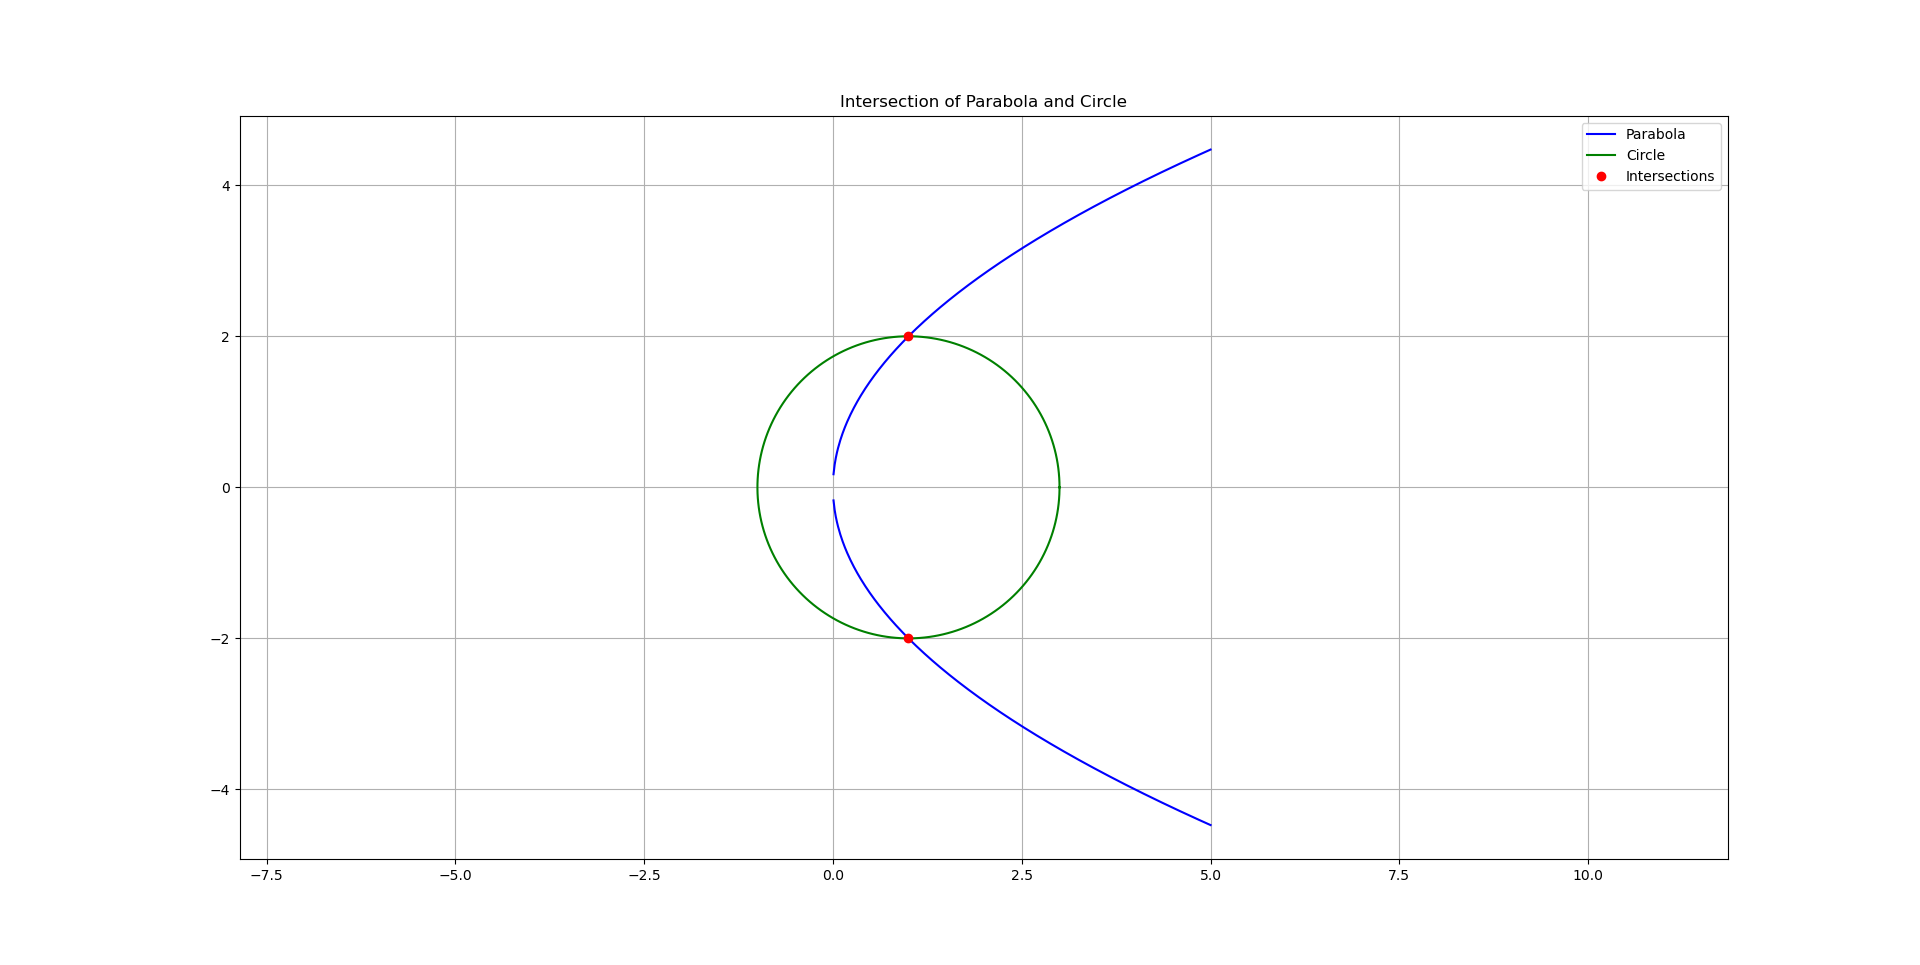
\includegraphics[width=0.8\linewidth]{./figs/Figure_1.png}
    \caption{Caption}
    \label{fig:placeholder}
\end{figure}





\end{document}